\section{Bewegung}
\label{sec:physik:bewegung}



Sicherlich habt Ihr schon einiges über Bewegung erfahren und schon Aufgaben gelöst, in denen zum Beispiel gefragt wird:\footnote{%
    Die Aufgabe werdet Ihr vermutlich mit Leichtigkeit lösen. Dennoch ist es ratsam, dass Ihr dieses Kapitel mit einer Begleitperson durchlest, die Eure fragen beantworten kann.}

\begin{exercise}
    Ein Zug fährt von Bonn mit \qty{100}{\km\per\hour} nach Stuttgart. Ein anderer Zug fährt zur gleichen Zeit los, aber mit \qty{200}{\km\per\hour} von Stuttgart nach Bonn. Wenn wir annehmen, die Entfernung über die Schiene ist \qty{300}{\km}, wie lange dauert es, bis die Züge sich begegnen?
    \begin{solution}
        Es dauert \qty{1}{\hour}.
    \end{solution}
\end{exercise}
Das werdet Ihr natürlich sofort sagen können -- aber, wenn wir Bewegung berechnen, müssen wir -- über die Formeln hinaus -- wissen, welchen Bezugspunkt man wählt. Setzt Euch mal hin und bewegt Euch nicht vom Fleck. Welche Geschwindigkeit habt Ihr dann? Die Antwort ist faszinierend:
\begin{itemize}
    \item Auf der Erdoberfläche ist Eure Geschwindigkeit \qty{0}{\km\per\hour}.
    \item Aufgrund der Erdrotation bewegt Ihr Euch aber mit etwa \qty{800}{\km\per\hour} (etwa \qty{220}{\meter\per\second}) um die Rotationsachse.
    \item Die Erde kreist um die Sonne mit etwa \qty{107000}{\km\per\hour}.
    \item Unser Sonnensystem bewegt sich in der Galaxy mit etwa \qty{864000}{\km\per\hour} (das sind \qty{240000}{\meter\per\second}).
\end{itemize}
Jetzt könntet Ihr natürlich zweifeln und sagen: ``wenn ich im Auto mit \qty{100}{\km\per\hour} um eine Kurve fahre, dann drückt es mich nach außen! Wieso fliege ich dann nicht weg, wenn ich mit \qty{800}{\km\per\hour} um die Erdachse drehe?'' Die Antwort liegt natürlich klar an der Erdanziehung. Diese Erdanziehung (in der Fachsprache: \emph{Gravitation}), weswegen auch die Tropfen auf den Boden fallen, wird mit der Konstante $g$ beschrieben. Ihr Wert ist $g = \qty{9,81}{\m\per\second^2}$. Tatsächlich ist das eine Beschleunigung. Fangen wir aber zuerst mit der sogenannten ``gleichmäßigen'' Bewegung an, in der Beschleunigung noch keine Rolle spielt.

%%%%%%%%%%%%%%%%%%%%%%%%%%%%%%%%%%%%%%%%%%%%%%%%%%%%%%%%%%%%%%%%%%%%%%%%%%%%%%%%%%%%%%%%%%%%%%%%%%%%%%%%%%%%%%%%%%%%%%%%%%%%%%%%%%%
\paragraph{Gleichmäßige Bewegung}

Um die Bewegung der Regentropfen zu berechnen, müssen wir mit Formeln arbeiten. Zunächst wollen wir dazu nur beschreiben, wie weit sich ein Objekt bei konstanter Geschwindigkeit (das nennt man ``gleichmäßig'') bewegt. Dazu hat der Physiker die Formel:
\begin{equation*}
    s = v\cdot t\,.
\end{equation*}
Diese Formel sagt: die Streck $s$, die ein Objekt mit der Geschwindigkeit $v$ in der Zeit $t$ zurücklegt, ist ``Geschwindigkeit mal Zeit'', also $v\cdot t$.\footnote{%
    Diese Variablennamen kommen aus dem Lateinischen, \emph{spatium} oder \emph{situs} für Strecke, \emph{velocitas} für Geschwindigkeit und \emph{tempus} für Zeit. Im Englischen benutzt man \emph{space}, \emph{velocity} und \emph{time}. Die Wahl dieser Buchstaben ist dennoch nur eine Konvention, das heißt eine Abmachung. Durch diese Abmachung ist es einfacher, den Sinn und Zweck einer physikalischen oder mathematischen Formel zu erkennen. Es existiert eine Vielzahl solcher Konvention -- Ihr werdet einige davon im Laufe der Schulzeit kennen lernen. Für das Volumen zum Beispiel wird das große $V$ verwendet. Eine der wichtigsten Konventionen kennt Ihr bestimmt schon: jeder weiß, was der griechische Buchstabe $\pi$ bedeutet -- nämlich die Kreiszahl.}

Wir wollen einmal die obige Übung mit dieser Formel ausdrücken. Dazu müssen wir die Formel ein bisschen erweitern -- den wir müssen betrachten, wie die Züge sich zueinander bewegen: was Ihr vorher im Kopf gemacht habt, müssen wir in die Formeln schreiben, nämlich den Bezugspunkt (das gleich gilt auch für den Regentropfen, der ja, wenn er anfängt zu fallen, nicht bei Höhe 0 anfängt). Dazu schreibt man
\begin{equation*}
    s = s_0 + v\cdot t\,,
\end{equation*}
wobei das $s_0$ die Position zur Zeit $t=0$ angibt.

Um nun die obige Aufgabe nachzurechenen, wählen wir Bonn als Bezugsort Bonn. Damit können wir die beiden Züge so beschreiben:
\begin{equation}
    \begin{split}
        s_1 &= v_1\cdot t \\
        s_2 &= d + v_2\cdot t\,.
    \end{split}
    \label{eq:physik:bewegung:zuege}
\end{equation}
Dabei berechnen wir die Entfernung von Bonn, $s_1$ ist die Entfernung von Bonn des Zugs der in Bonn startet, $s_2$ die des Zugs, der in Stuttgart startet. Bonn und Stuttgart haben die Entfernung $d$. Die Zuggeschwindigkeiten sind $v_1$ des Bonner Zuges und $v_2$ des Stuttgarter Zuges. In den Formeln steckt ein kleiner Stolperstein, der in Klassenarbeiten schnell zu einem Leichtsinnsfehler führen kann: da wir Bonn als Bezugsort ausgewählt haben, fährt der Bonner Zug mit $v_1 = \qty{100}{\km\per\hour}$, der Stuttgarter Zug aber mit $v_2 = -\qty{200}{\km\per\hour}$! Mit den Formeln können wir nun rechnerisch lösen, in dem wir $s_1$ mit $s_2$ gleichsetzen, also genau dann, wenn die Entfernung beider Züge von Bonn gleich ist, sie sich also begegnen:
\begin{align*}
    s_1 &= s_2 && \iff\\
    v_1\cdot t &= d + v_2\cdot t\,, &&
\end{align*} 
Bei mathematischen Formeln heißt der Doppelpfeil ($\iff$) so viel wie ``genau dann, wenn''. Nun müssen wir so umformen, dass am Ende die Zeit $t$, die wir ja noch nicht kennen, links als Ergebnis stehen bleibt:
\begin{align*}
    v_1\cdot t &= d + v_2\cdot t && \iff\\
    v_1\cdot t - v_2\cdot t &= d && \iff\\
    (v_1-v_2)\cdot t &= d && \iff\\
    t &= \frac{d}{v_1-v_2}\,,
\end{align*} 
mit Einsetzen der Werte erhalten wir
\begin{align*}
    t &= \frac{\qty{300}{\km}}{\qty{100}{\km\per\hour} - (-\qty{200}{\km\per\hour})} && \iff \\
    t &= \frac{\qty{300}{\km}}{\qty{100}{\km\per\hour} + \qty{200}{\km\per\hour}} && \iff \\
    t &= \frac{\qty{300}{\km}}{\qty{300}{\km\per\hour}} = \qty{1}{\hour} \,.&&\\
\end{align*} 

Wir können das gleiche Ergebnis aber auch mit einem Diagramm lösen.
\begin{figure}[h]
    % GNUPLOT: LaTeX picture with Postscript
\begingroup
  \makeatletter
  \providecommand\color[2][]{%
    \GenericError{(gnuplot) \space\space\space\@spaces}{%
      Package color not loaded in conjunction with
      terminal option `colourtext'%
    }{See the gnuplot documentation for explanation.%
    }{Either use 'blacktext' in gnuplot or load the package
      color.sty in LaTeX.}%
    \renewcommand\color[2][]{}%
  }%
  \providecommand\includegraphics[2][]{%
    \GenericError{(gnuplot) \space\space\space\@spaces}{%
      Package graphicx or graphics not loaded%
    }{See the gnuplot documentation for explanation.%
    }{The gnuplot epslatex terminal needs graphicx.sty or graphics.sty.}%
    \renewcommand\includegraphics[2][]{}%
  }%
  \providecommand\rotatebox[2]{#2}%
  \@ifundefined{ifGPcolor}{%
    \newif\ifGPcolor
    \GPcolortrue
  }{}%
  \@ifundefined{ifGPblacktext}{%
    \newif\ifGPblacktext
    \GPblacktexttrue
  }{}%
  % define a \g@addto@macro without @ in the name:
  \let\gplgaddtomacro\g@addto@macro
  % define empty templates for all commands taking text:
  \gdef\gplbacktext{}%
  \gdef\gplfronttext{}%
  \makeatother
  \ifGPblacktext
    % no textcolor at all
    \def\colorrgb#1{}%
    \def\colorgray#1{}%
  \else
    % gray or color?
    \ifGPcolor
      \def\colorrgb#1{\color[rgb]{#1}}%
      \def\colorgray#1{\color[gray]{#1}}%
      \expandafter\def\csname LTw\endcsname{\color{white}}%
      \expandafter\def\csname LTb\endcsname{\color{black}}%
      \expandafter\def\csname LTa\endcsname{\color{black}}%
      \expandafter\def\csname LT0\endcsname{\color[rgb]{1,0,0}}%
      \expandafter\def\csname LT1\endcsname{\color[rgb]{0,1,0}}%
      \expandafter\def\csname LT2\endcsname{\color[rgb]{0,0,1}}%
      \expandafter\def\csname LT3\endcsname{\color[rgb]{1,0,1}}%
      \expandafter\def\csname LT4\endcsname{\color[rgb]{0,1,1}}%
      \expandafter\def\csname LT5\endcsname{\color[rgb]{1,1,0}}%
      \expandafter\def\csname LT6\endcsname{\color[rgb]{0,0,0}}%
      \expandafter\def\csname LT7\endcsname{\color[rgb]{1,0.3,0}}%
      \expandafter\def\csname LT8\endcsname{\color[rgb]{0.5,0.5,0.5}}%
    \else
      % gray
      \def\colorrgb#1{\color{black}}%
      \def\colorgray#1{\color[gray]{#1}}%
      \expandafter\def\csname LTw\endcsname{\color{white}}%
      \expandafter\def\csname LTb\endcsname{\color{black}}%
      \expandafter\def\csname LTa\endcsname{\color{black}}%
      \expandafter\def\csname LT0\endcsname{\color{black}}%
      \expandafter\def\csname LT1\endcsname{\color{black}}%
      \expandafter\def\csname LT2\endcsname{\color{black}}%
      \expandafter\def\csname LT3\endcsname{\color{black}}%
      \expandafter\def\csname LT4\endcsname{\color{black}}%
      \expandafter\def\csname LT5\endcsname{\color{black}}%
      \expandafter\def\csname LT6\endcsname{\color{black}}%
      \expandafter\def\csname LT7\endcsname{\color{black}}%
      \expandafter\def\csname LT8\endcsname{\color{black}}%
    \fi
  \fi
    \setlength{\unitlength}{0.0500bp}%
    \ifx\gptboxheight\undefined%
      \newlength{\gptboxheight}%
      \newlength{\gptboxwidth}%
      \newsavebox{\gptboxtext}%
    \fi%
    \setlength{\fboxrule}{0.5pt}%
    \setlength{\fboxsep}{1pt}%
    \definecolor{tbcol}{rgb}{1,1,1}%
\begin{picture}(6800.00,4520.00)%
    \gplgaddtomacro\gplbacktext{%
      \csname LTb\endcsname%%
      \put(629,697){\makebox(0,0)[r]{\strut{}$0$}}%
      \csname LTb\endcsname%%
      \put(629,1209){\makebox(0,0)[r]{\strut{}$50$}}%
      \csname LTb\endcsname%%
      \put(629,1721){\makebox(0,0)[r]{\strut{}$100$}}%
      \csname LTb\endcsname%%
      \put(629,2233){\makebox(0,0)[r]{\strut{}$150$}}%
      \csname LTb\endcsname%%
      \put(629,2745){\makebox(0,0)[r]{\strut{}$200$}}%
      \csname LTb\endcsname%%
      \put(629,3257){\makebox(0,0)[r]{\strut{}$250$}}%
      \csname LTb\endcsname%%
      \put(629,3769){\makebox(0,0)[r]{\strut{}$300$}}%
      \csname LTb\endcsname%%
      \put(629,4282){\makebox(0,0)[r]{\strut{}$350$}}%
      \csname LTb\endcsname%%
      \put(721,479){\makebox(0,0){\strut{}$0$}}%
      \csname LTb\endcsname%%
      \put(1492,479){\makebox(0,0){\strut{}$0.2$}}%
      \csname LTb\endcsname%%
      \put(2263,479){\makebox(0,0){\strut{}$0.4$}}%
      \csname LTb\endcsname%%
      \put(3034,479){\makebox(0,0){\strut{}$0.6$}}%
      \csname LTb\endcsname%%
      \put(3806,479){\makebox(0,0){\strut{}$0.8$}}%
      \csname LTb\endcsname%%
      \put(4577,479){\makebox(0,0){\strut{}$1$}}%
      \csname LTb\endcsname%%
      \put(5348,479){\makebox(0,0){\strut{}$1.2$}}%
      \csname LTb\endcsname%%
      \put(6119,479){\makebox(0,0){\strut{}$1.4$}}%
    }%
    \gplgaddtomacro\gplfronttext{%
      \csname LTb\endcsname%%
      \put(5777,4085){\makebox(0,0)[r]{\strut{}Zug Bonn $\rightarrow$ Stuttgart}}%
      \csname LTb\endcsname%%
      \put(5777,3868){\makebox(0,0)[r]{\strut{}Zug Stuttgart $\rightarrow$ Bonn}}%
      \csname LTb\endcsname%%
      \put(177,2489){\rotatebox{-270.00}{\makebox(0,0){\strut{}Entfernung von Bonn [km]}}}%
      \csname LTb\endcsname%%
      \put(3613,152){\makebox(0,0){\strut{}Zeit t [h]}}%
    }%
    \gplbacktext
    \put(0,0){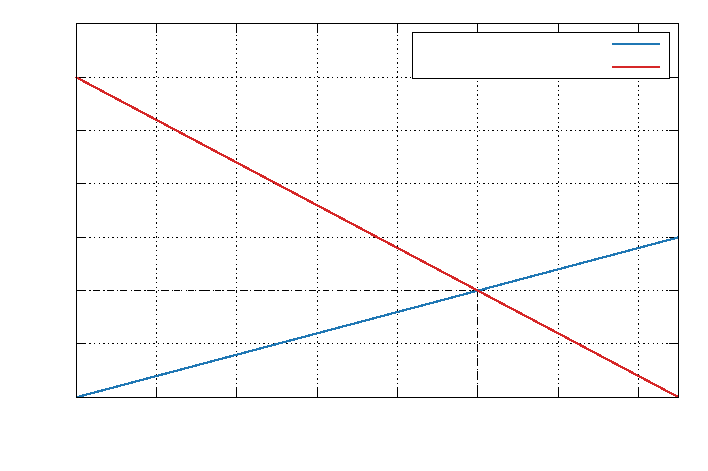
\includegraphics[width={340.00bp},height={226.00bp}]{physik/images/zuege}}%
    \gplfronttext
  \end{picture}%
\endgroup

    \caption{Entfernung der Züge von Bonn in der Darstellung eines Diagramms. Der Punkt an dem sich die Züge treffen ist der Schnittpunkt der roten und blauen Linie.}
    \label{img:physik:bewegung:zuege}
\end{figure}
Aus dem Diagramm in Abb.~\ref{img:physik:bewegung:zuege} kann man mehrere Dinge ablesen, die wir natürlich auch mit den Formeln berechnen können: 1. Eine vertikal Linie vom Schnittpunkt beider Geraden auf die Zeitachse zeigt uns wann beide Züge sich treffen (nach \qty{1}{\hour}). 2. Eine horizontale Linie vom Schnittpunkt beider Gerade zur Entfernungsachse zeigt uns wo die beiden Züge sich treffen (in einer Entfernng \qty{100}{km} von Bonn entfernt). 3. Wenn der Zug aus Stuttgart Bonn erreicht, hat der Zug aus Bonn erst die Hälfte seiner Streck zurückgelegt (nämlich \qty{150}{\km}).

Um dies zu berechnen wollen wir die Notation (das heißt: die Schreibweise) etwas verfeinern und schreiben die Beziehung von Strecke zu Zeit so:\footnote{%
    Die Notation, so wie auch musikalische Noten, hat sich über viele Jahrhunderte entwickelt. Dadurch ist die Mathematik zu einer universellen (also weltweiten) Sprache geworden, die jeder verstehen kann. Den kleinen Ausschnitt, den wir hier zeigen, versteht jeder, der ein bisschen Mathe kann.}
\begin{equation*}
    s(t) = s_0 + v\cdot t\,.
\end{equation*}
Für den Leser wird damit deutlich: die Zeit $t$ ist eine Variable während die Geschwindigkeit $v$ und der Startpunkt $s_0$ feste Werte, man nennt sie Konstanten, sind. Das ist genau dasselbe wie in der Programmiersprache C.\footnote{%
    In der Tat haben viele Programmiersprachen
    } Da würden wir schreiben:
\begin{code}[numbers=none]
    #define S_0 300
    #define V -200
    double strecke(double t) {
        return S_0 + V * t;
    }
\end{code}
Damit schreiben wir die Gleichung (\ref{eq:physik:bewegung:zuege}) folgendermaßen:
\begin{equation}
    \begin{split}
        s_1(t) &= v_1\cdot t \\
        s_2(t) &= d + v_2\cdot t\,.
    \end{split}
\end{equation}
Ein weiteres Detail ist die Zeit, bei der sich beide Züge treffen: man würde hier einen anderen Namen wählen, denn $t = \qty{1}{\hour}$ würde bedeuten, dass auch $t$ zu einer Konstanten wird, wir schreiben daher:
\begin{equation*}
    t_\textrm{x} = \qty{1}{\hour} \,.
\end{equation*}
Mit dieser Schreibweise berechnen wir den Abstand von Bonn zu dem Zeitpunkt $t_\textrm{x}$ mit
\begin{equation*}
    s_1(t_\textrm{x}) = v_1\cdot t_\textrm{x} = \cdots = \qty{100}{\km} \,.
\end{equation*}

%%%%%%%%%%%%%%%%%%%%%%%%%%%%%%%%%%%%%%%%%%%%%%%%%%%%%%%%%%%%%%%%%%%%%%%%%%%%%%%%%%%%%%%%%%%%%%%%%%%%%%%%%%%%%%%%%%%%%%%%%%%%%%%%%%%
\paragraph{Newton und die Kraft}

\begin{marginfigure}%
    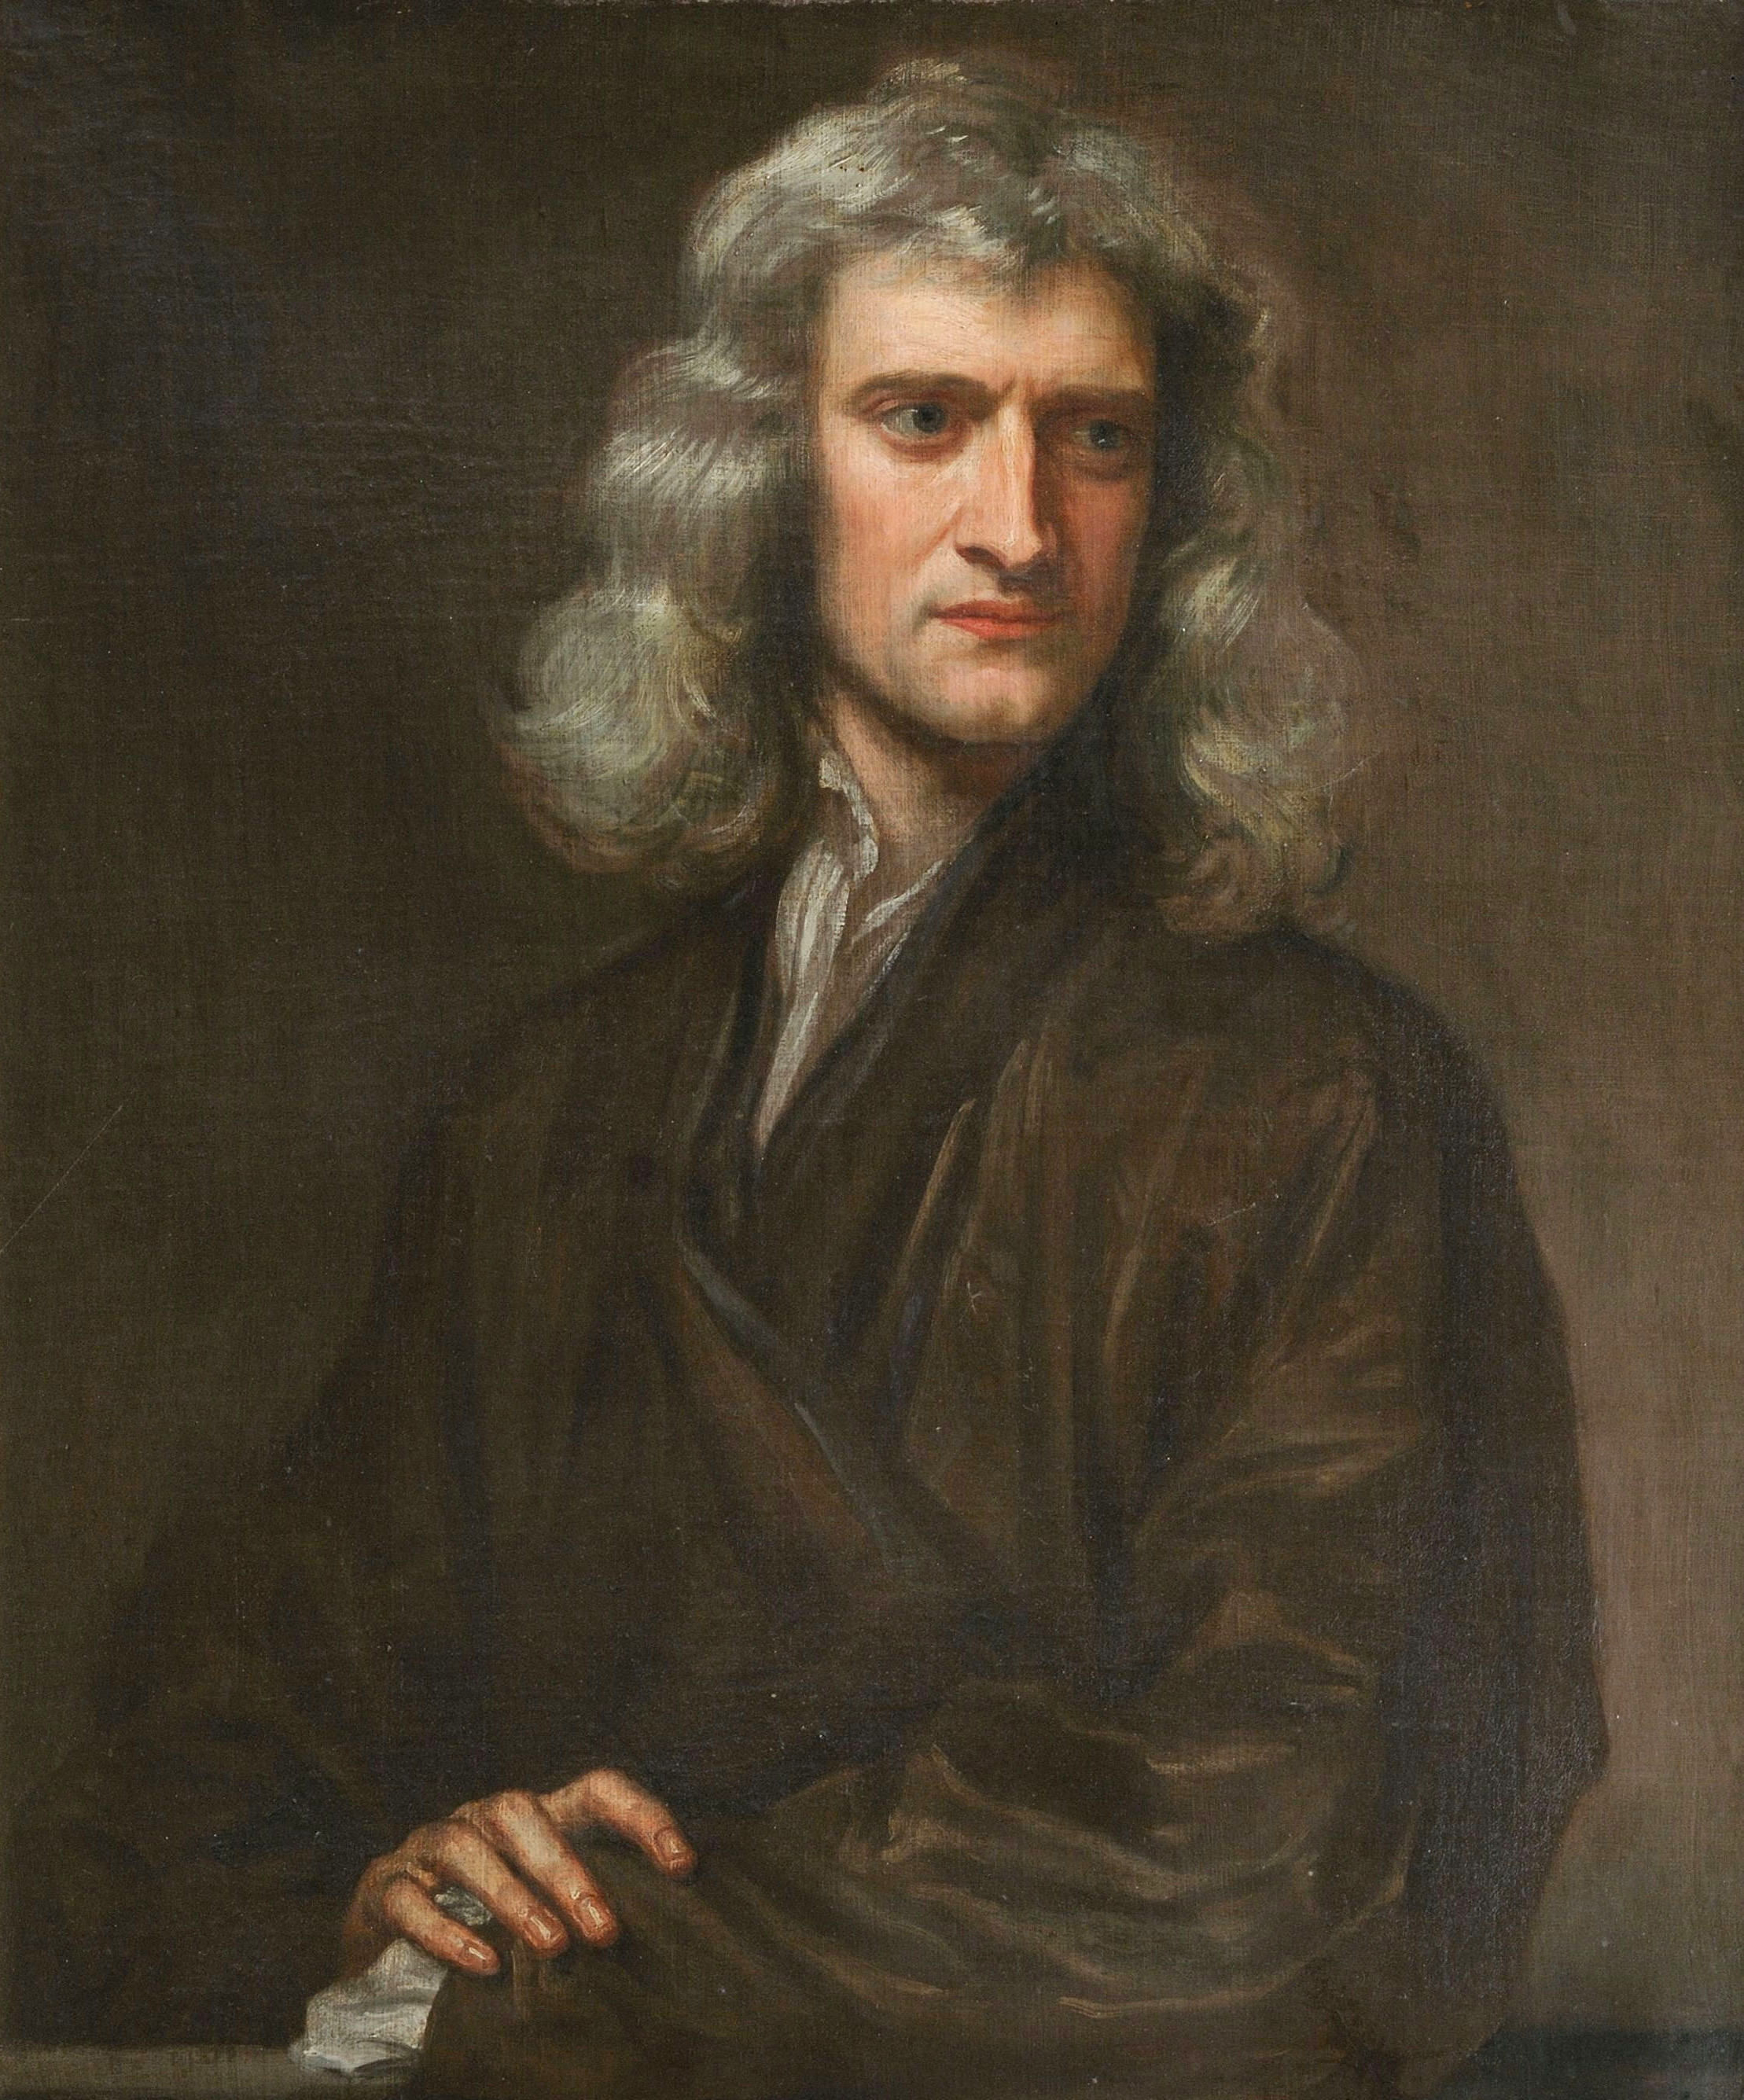
\includegraphics[width=\linewidth]{images/Portrait_of_Sir_Isaac_Newton,_1689_(brightened).jpg}
    \caption{Sir Isaac Newton, 1643--1727. (Gemälde von Godfrey Kneller, 1689. Das Bild ist gemeinfrei / Allgemeingut, Wikimedia Commons)}%
    \label{fig:physik:newton}
\end{marginfigure}%
Sir Newton saß in seinem Garten unter einem Apfelbaum, als er einen Apfel fallen sah. Augenzeugen berichten, dass er tief in Gedanken versunken war. Der fallende Apfel löste eine Gedankenkette aus und er fragte sich: Warum fällt der Apfel immer gerade nach unten -- und warum fällt der Mond nicht auch auf die Erde? Die Schlüsse, die er zog, haben noch immer Gültigkeit. 

Aus diesen Gedanken sind drei Naturgesetze entstanden, die er 1687 veröffentlichte (und noch immer gelehrt werden):
\begin{description}
\item[Trägheit] Ein Körper, auf den keine Kraft wirkt, behält seinen Bewegungszustand bei.
\item[Kraft und Beschleunigung] Kraft ist gleich Masse mal Beschleunigung.
\item[Wechselwirkung] ``actio'' ist gleich ``reactio'' -- Übt ein Körper A auf einen anderen Körper B eine Kraft aus (actio), so wirkt eine gleich große, aber entgegen gerichtete Kraft von Körper B auf Körper A (reactio).
\end{description}

\vskip\baselineskip

\noindent
Schauen wir uns die drei Gesetze einmal genauer an:\footnote{%
    FIXME Aristoteles, Descartes, Euler, und so weiter, haben schon vor Newton daran gearbeitet. Übrigens, bis vor 100 Jahren sagte man nicht Physiker, sondern Naturphilosophen... Newton hat als Erster erkannt, dass die Kraft, die einen Apfel fallen lässt, dieselbe ist, die die Planeten bewegt... Streng genommen sind es Axiom...}

\vskip\baselineskip

\noindent
\textbf{Trägheit}\footnote{%
    Das 1.\ Newtonsche Gesetz wird als \textbf{Trägheitsprinzip} bezeichnet.}\\
Den Begriff Trägheit kennt Ihr natürlich Wenn Ihr träge seid (sprich: einfach keine Lust habt, etwas zu tun), bleibt Ihr sitzen und verändert Euren ``Bewegungszustand'' nicht. Aber genau das meint Newton nicht und es ist sehr schwer zu verstehen, weil wir es tatsächlich nicht beobachten können. Was Newton meint, ist, dass ein Körper -- auf den keine Kräfte wirken -- seine Geschwindigkeit beibehält. Auf ein Auto übertragen hieße das: wenn man in der Stadt mit \qty{30}{\km\per\hour} fährt und man den Fuß vom Gas nimmt (der Motor also keine Kraft mehr an die Räder weitergibt) dann fährt das Auto mit \qty{30}{\km\per\hour} bis in alle Unendlichkeit so schnell weiter, bis man die Bremse betätigt. Die Krux\footnote{%
    Krux (von lateinisch \emph{crux}, das Kreuz) bedeutet so viel wie `Schwierigkeit' oder `Haken'. Den Begriff könnt Ihr Euch merken, falls Ihr einmal Scrabble spielt und nicht wisst, was Ihr mit einem 'X' machen sollt.}
daran ist, das wir daran gewöhnt sind, Reibung nicht als ``Kraft'' zu verstehen. Im physikalischen -- und damit Newtons -- Sinn, ist aber Reibung eine Kraft. Bei einem Auto sind das zum Beispiel die Reifen auf der Straße. Aber auch der sogenannte Luftwiderstand, der vor allem für unsere Regensimulation eine Rolle spielt -- und den wir später noch genauer anschauen werden, ist ``Reibung'': eine Kraft. Was Newton also meint: ein Körper, auf den keine Kraft einwirkt (weder Anziehungskraft noch Reibung) bewegt sich \emph{gleichmäßig} weiter (siehe vorhergehendes Kapitel -- $v=0$, also ``stehen bleiben'', gehört dazu). 
% TODO "weil wir es tatsächlich nicht beobachten können" sollte erklärt werden...

\vskip\baselineskip

\noindent
\textbf{Kraft und Beschleunigung}\footnote{%
    Das 2.\ Newtonsche Gesetz wird als \textbf{Aktionsprinzip} bezeichnet.}\\
Vom Fußballspielen wisst Ihr natürlich, dass, wenn Ihr doppelt so stark den Ball tretet, dass der Ball dann auch gefühlt doppelt so weit fliegt. Aber warum ist denn nun die Kraft gleich Masse mal Beschleunigung. 

Denkt mal an eine Feder. Wenn Ihr an einer Feder zieht, verlängert sie sich. Zieht Ihr doppelt so stark, verlängert sie sich doppelt so weit. Eine Feder ist also ein prima Kraftmesser. Hängt man ein Gewicht (zum Beispiel ein 1-kg-Stück) an die Feder, verlängert sie sich um eine bestimmte Strecke. Hängt man zwei gleiche Gewichte daran, verlängert sie sich doppelt so weit. Die Gewichte ziehen also doppelt so stark an der Feder.

Jetzt stellen wir uns vor, wir fliegen zum Mond. Dort ist die Anziehungskraft nur ein Sechstel so groß wie auf der Erde. Was beobachten wir? Die Feder verlängert sich nur noch ein Sechstel so weit. Das Gewicht zieht also nur noch ein Sechstel so stark.

Was passiert nun, wenn wir das Gewicht fallen lassen? Auf dem Mond fällt es sechs Mal langsamer zu Boden als auf der Erde. Die Beschleunigung ist also auch nur ein Sechstel so groß -- und jetzt kommt der Trick: Was gleich bleibt, ist die Masse! Denn Ihr nehmt ja nichts von den Gewichten weg und tut auch nichts hinzu. Das Verhältnis von Kraft zu Beschleunigung bleibt also gleich. Genau das steckt in der Formel $F=m\cdot a$: die Kraft ist das Produkt aus Masse und Beschleunigung.

(Und dass ein Hammer und eine Feder im Vakuum sogar gleich schnell fallen, obwohl sie unterschiedlich schwer sind -- das schauen wir uns später bei der Reibung an.)

\vskip\baselineskip

\noindent
\textbf{Wechselwirkung}\footnote{%
    Das 3.\ Newtonsche Gesetz wird als \textbf{Wechselwirkungsprinzip} bezeichnet}\\
Ihr könntet Euch jetzt fragen: wenn wir auf der Erde stehen und die Erde eine Gewichtskraft auf mich ausübt, übe ich dann auch die gleich Kraft auf die Erde aus? Die Antwort ist kaum zu glauben: Ja! Es wird sogar noch unglaublicher: Wenn Ihr von der Erde wegspringt, beschleunigt Ihr nicht nur Euch selbst, sondern auch die Erde mit der gleichen Kraft, mit der Ihr losgesprungen seid.\footnote{%
    Falls Ihr Euch fragt, ob man das Messen könnte, dann müsst Ihr wissen, dass die Erde ungefähr eine Masse von \qty{6e24}{\kg} hat -- das ist die Zahl 6 mit 24 Nullen. Selbst wenn alle Menschen sich auf einer Seite der Erde zusammenfinden und gleichzeitig hochspringen, ist das Verhältnis so enorm, dass man es nicht feststellen könnte.}

Am besten kann man sich dieses Wechselwirkungsprinzip vorstellen, in dem wir uns fragen, wie eine Rakete zum Mond fliegen kann. Eine Rakete ist tatsächlich nichts anderes als ein riesiger Motor, der heiße Gase mit voller Wucht nach unten ausstößt. Die Kraft, mit der die Gase ausgestoßen werden (actio), drücken die Rakete mit derselben Kraft in die entgegengesetzte Richtung (reactio). Die Rakete muss also gar nicht an etwas ``ziehen'', um nach oben zu kommen -- sie erreicht das, indem sie etwas nach unten wirft. Der Ausstoß muss allerdings so groß sein, dass die Rakete auch der Erdanziehung ``entfliehen'' kann. Ohne dieses Gesetz (das man deshalb auch das Rückstoßprinzip nennt) wäre die Menschheit nie in den Weltraum gekommen.

%%%%%%%%%%%%%%%%%%%%%%%%%%%%%%%%%%%%%%%%%%%%%%%%%%%%%%%%%%%%%%%%%%%%%%%%%%%%%%%%%%%%%%%%%%%%%%%%%%%%%%%%%%%%%%%%%%%%%%%%%%%%%%%%%%%
\paragraph{Beschleunigte Bewegung}

Für die beschleunigte Bewegung gibt es zwei wichtige Gleichungen:
\begin{align}
    v(t) &= v_0 + a\cdot t \\
    s(t) &= s_0 + \frac12 a\cdot t^2 \,.
\end{align}
Hier sind $v_0$ und $s_0$ die anfängliche Geschwindigkeit und Strecke, $a$ die Beschleunigung und wieder $t$ die Zeit.\footnote{%
    Diese Variablennamen kommen aus dem Lateinischen, \emph{acceleratio} für Beschleunigung und \emph{gravitas} (Schwere) für Erdbeschleunigung. Im Englischen benutzt man \emph{acceleration} und \emph{gravity}.}
Im vorhergehenden Abschnitt haben wir ja gesehen, dass Objekte auf der Erde durch die Erdanziehung in Richtung Erde beschleunigt werden. Die Beschleunigung, die auf eine Tropfen wirkt, ist die Erdbeschleunigung, die durch $g$ beschrieben wird. Diese Erdbeschleunigung\footnote{%
    Die Kraft, mit der ein Objekt angezogen wird, nennt man ganz allgemein Gravitation. Alle Objekt -- die Masse haben -- ziehen sich durch Gravitation an. Erstaunlicherweise sind sich die Physiker noch nicht im Klaren, was Gravitation tatsächlich ist. Das gilt übrigens auch in anderen Bereichen, in denen Physiker Dinge zwar sehr genau mathematisch beschreiben und berechnen können -- den Ursache dafür aber noch nicht kennen. Der Autor möchte zu Gravitation auch anmerken, dass eine Gruppe Mathematiker 2026 darstellen konnte, dass -- entgegen bisheriger Lehrmeinung -- die Gravition keine Grundkraft ist.}
    % FIXME maybe too much for kids ("Grundkraft"), evtl. Studio weglassen
ist (fast) eine Konstante, die wir mit $g = \qty{9,81}{\meter\per\second^2}$ verwenden können.

Um herauszufinden, was es bedeutet, wenn ein Körper zur Erde fällt betrachten wir ein Sandkorn. Starke Winde können den Sand der Sahara über Hunderte Kilometer weit  bis zu einer Höhe von \qty{10}{\km} um die Erde tragen (der Autor hat diesen roten Sand schon in seiner Kindheit in Deutschland zur Erde fallen sehen). 
% TODO vll. Fußnote über "jet streams"
Wenn ein Sandkorn nun aus dieser Höhe mit fällt, beschrieben durch die genannten Formeln, machen wir einigen aufschlussreiche Feststellungen.
\begin{figure}[h]
    % GNUPLOT: LaTeX picture with Postscript
\begingroup
  \makeatletter
  \providecommand\color[2][]{%
    \GenericError{(gnuplot) \space\space\space\@spaces}{%
      Package color not loaded in conjunction with
      terminal option `colourtext'%
    }{See the gnuplot documentation for explanation.%
    }{Either use 'blacktext' in gnuplot or load the package
      color.sty in LaTeX.}%
    \renewcommand\color[2][]{}%
  }%
  \providecommand\includegraphics[2][]{%
    \GenericError{(gnuplot) \space\space\space\@spaces}{%
      Package graphicx or graphics not loaded%
    }{See the gnuplot documentation for explanation.%
    }{The gnuplot epslatex terminal needs graphicx.sty or graphics.sty.}%
    \renewcommand\includegraphics[2][]{}%
  }%
  \providecommand\rotatebox[2]{#2}%
  \@ifundefined{ifGPcolor}{%
    \newif\ifGPcolor
    \GPcolortrue
  }{}%
  \@ifundefined{ifGPblacktext}{%
    \newif\ifGPblacktext
    \GPblacktexttrue
  }{}%
  % define a \g@addto@macro without @ in the name:
  \let\gplgaddtomacro\g@addto@macro
  % define empty templates for all commands taking text:
  \gdef\gplbacktext{}%
  \gdef\gplfronttext{}%
  \makeatother
  \ifGPblacktext
    % no textcolor at all
    \def\colorrgb#1{}%
    \def\colorgray#1{}%
  \else
    % gray or color?
    \ifGPcolor
      \def\colorrgb#1{\color[rgb]{#1}}%
      \def\colorgray#1{\color[gray]{#1}}%
      \expandafter\def\csname LTw\endcsname{\color{white}}%
      \expandafter\def\csname LTb\endcsname{\color{black}}%
      \expandafter\def\csname LTa\endcsname{\color{black}}%
      \expandafter\def\csname LT0\endcsname{\color[rgb]{1,0,0}}%
      \expandafter\def\csname LT1\endcsname{\color[rgb]{0,1,0}}%
      \expandafter\def\csname LT2\endcsname{\color[rgb]{0,0,1}}%
      \expandafter\def\csname LT3\endcsname{\color[rgb]{1,0,1}}%
      \expandafter\def\csname LT4\endcsname{\color[rgb]{0,1,1}}%
      \expandafter\def\csname LT5\endcsname{\color[rgb]{1,1,0}}%
      \expandafter\def\csname LT6\endcsname{\color[rgb]{0,0,0}}%
      \expandafter\def\csname LT7\endcsname{\color[rgb]{1,0.3,0}}%
      \expandafter\def\csname LT8\endcsname{\color[rgb]{0.5,0.5,0.5}}%
    \else
      % gray
      \def\colorrgb#1{\color{black}}%
      \def\colorgray#1{\color[gray]{#1}}%
      \expandafter\def\csname LTw\endcsname{\color{white}}%
      \expandafter\def\csname LTb\endcsname{\color{black}}%
      \expandafter\def\csname LTa\endcsname{\color{black}}%
      \expandafter\def\csname LT0\endcsname{\color{black}}%
      \expandafter\def\csname LT1\endcsname{\color{black}}%
      \expandafter\def\csname LT2\endcsname{\color{black}}%
      \expandafter\def\csname LT3\endcsname{\color{black}}%
      \expandafter\def\csname LT4\endcsname{\color{black}}%
      \expandafter\def\csname LT5\endcsname{\color{black}}%
      \expandafter\def\csname LT6\endcsname{\color{black}}%
      \expandafter\def\csname LT7\endcsname{\color{black}}%
      \expandafter\def\csname LT8\endcsname{\color{black}}%
    \fi
  \fi
    \setlength{\unitlength}{0.0500bp}%
    \ifx\gptboxheight\undefined%
      \newlength{\gptboxheight}%
      \newlength{\gptboxwidth}%
      \newsavebox{\gptboxtext}%
    \fi%
    \setlength{\fboxrule}{0.5pt}%
    \setlength{\fboxsep}{1pt}%
    \definecolor{tbcol}{rgb}{1,1,1}%
\begin{picture}(6800.00,4520.00)%
    \gplgaddtomacro\gplbacktext{%
      \colorrgb{0.12,0.47,0.71}%%
      \put(812,697){\makebox(0,0)[r]{\strut{}$0$}}%
      \colorrgb{0.12,0.47,0.71}%%
      \put(812,1380){\makebox(0,0)[r]{\strut{}$2000$}}%
      \colorrgb{0.12,0.47,0.71}%%
      \put(812,2062){\makebox(0,0)[r]{\strut{}$4000$}}%
      \colorrgb{0.12,0.47,0.71}%%
      \put(812,2745){\makebox(0,0)[r]{\strut{}$6000$}}%
      \colorrgb{0.12,0.47,0.71}%%
      \put(812,3428){\makebox(0,0)[r]{\strut{}$8000$}}%
      \colorrgb{0.12,0.47,0.71}%%
      \put(812,4111){\makebox(0,0)[r]{\strut{}$10000$}}%
      \csname LTb\endcsname%%
      \put(904,479){\makebox(0,0){\strut{}$0$}}%
      \csname LTb\endcsname%%
      \put(1889,479){\makebox(0,0){\strut{}$10$}}%
      \csname LTb\endcsname%%
      \put(2874,479){\makebox(0,0){\strut{}$20$}}%
      \csname LTb\endcsname%%
      \put(3859,479){\makebox(0,0){\strut{}$30$}}%
      \csname LTb\endcsname%%
      \put(4844,479){\makebox(0,0){\strut{}$40$}}%
      \csname LTb\endcsname%%
      \put(5830,479){\makebox(0,0){\strut{}$50$}}%
      \colorrgb{0.84,0.15,0.16}%%
      \put(5921,697){\makebox(0,0)[l]{\strut{}$0$}}%
      \colorrgb{0.84,0.15,0.16}%%
      \put(5921,1414){\makebox(0,0)[l]{\strut{}$100$}}%
      \colorrgb{0.84,0.15,0.16}%%
      \put(5921,2131){\makebox(0,0)[l]{\strut{}$200$}}%
      \colorrgb{0.84,0.15,0.16}%%
      \put(5921,2848){\makebox(0,0)[l]{\strut{}$300$}}%
      \colorrgb{0.84,0.15,0.16}%%
      \put(5921,3565){\makebox(0,0)[l]{\strut{}$400$}}%
      \colorrgb{0.84,0.15,0.16}%%
      \put(5921,4282){\makebox(0,0)[l]{\strut{}$500$}}%
    }%
    \gplgaddtomacro\gplfronttext{%
      \csname LTb\endcsname%%
      \put(5102,4085){\makebox(0,0)[r]{\strut{}Höhe}}%
      \csname LTb\endcsname%%
      \put(5102,3868){\makebox(0,0)[r]{\strut{}Geschwindigkeit}}%
      \csname LTb\endcsname%%
      \put(5102,3650){\makebox(0,0)[r]{\strut{}Schallmauer}}%
      \colorrgb{0.12,0.47,0.71}%%
      \put(177,2489){\rotatebox{-270.00}{\makebox(0,0){\strut{}Höhe h [m]}}}%
      \colorrgb{0.84,0.15,0.16}%%
      \put(6396,2489){\rotatebox{-270.00}{\makebox(0,0){\strut{}Geschwindigkeit v [m/s]}}}%
      \csname LTb\endcsname%%
      \put(3367,152){\makebox(0,0){\strut{}Zeit t [s]}}%
    }%
    \gplbacktext
    \put(0,0){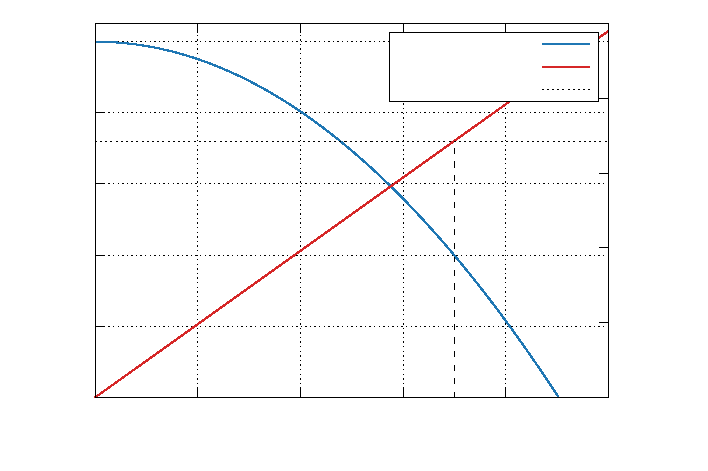
\includegraphics[width={340.00bp},height={226.00bp}]{physik/images/freierfall}}%
    \gplfronttext
  \end{picture}%
\endgroup

    \caption{Der freie Fall eines Sandkorns aus 10 km Höhe (ohne Luftwiderstand). Die blaue Linie zeigt die Höhe, die rote Linie die Geschwindigkeit. Nach etwa 35 Sekunden (gestrichelte Linie) durchbricht das Sandkorn die Schallmauer (gepunktete Linie).}
    \label{fig:physik:bewegung:sandkorn}
\end{figure}
Die Flugstrecke und Geschwindigkeit dieses Sandkorns werden in Abb.~\ref{fig:physik:bewegung:sandkorn} gezeigt. Da sehen wir, dass das Sandkorn nach etwa \qty{35}{s} die Schallmauer durchbricht (um die \qty{1200}{\km\per\hour}) und schon \qty{6}{\km} weit geflogen ist. Nach \qty{45}{\second} schlägt es dann mit eine Geschwindigkeit von etwa \qty{1620}{\km\per\hour} auf den Boden. 

Solch eine Geschwindigkeit würde selbst für ein Sandkorn zu schweren Verletzungen führen -- in der Realität wird ein Sandkorn aber höchstens mit \qty{15}{\km\per\hour} zu Boden fallen, denn die obigen Formeln haben einen ``kleinen'' Nachteil: sie gelten nur im Vakuum, also ohne Luftreibung. Da wir später aber unser ``Regensimulation'' zu programmieren wollen, dass sie natürlich aussieht, müssen wir uns mit dem Thema Reibung befassen.

%%%%%%%%%%%%%%%%%%%%%%%%%%%%%%%%%%%%%%%%%%%%%%%%%%%%%%%%%%%%%%%%%%%%%%%%%%%%%%%%%%%%%%%%%%%%%%%%%%%%%%%%%%%%%%%%%%%%%%%%%%%%%%%%%%%
\paragraph{Reibung}



Die Kraft auf einen Körper...
\begin{equation}
    F_\textrm{w}(v) = \frac12 \cdot c_\textrm{w} \cdot A \cdot \varrho \cdot v^2 \,.
\end{equation}
mit 
\begin{description}
    \item[$c_\textrm{w}$]Der Luftwiderstandsbeiwert (formabhängig, "Windschnittigkeit"). 
    \item[$A$] Die Querschnittsfläche des Körpers senkrecht zur Strömung. 
    \item[$\varrho$] Die Dichte der Luft. 
    \item[$v$] Die Geschwindigkeit des Körpers relativ zur Luft. 
\end{description}
% c_w Sandkorn, etwa 0.4
% Luftdichte (Standard) 1,225 kg/m^3

% siehe youtube Apollo 15 (Hammer & Feder)
% -> https://nssdc.gsfc.nasa.gov/planetary/image/AS15_Ham_feath_drop.mp4

%%%%%%%%%%%%%%%%%%%%%%%%%%%%%%%%%%%%%%%%%%%%%%%%%%%%%%%%%%%%%%%%%%%%%%%%%%%%%%%%%%%%%%%%%%%%%%%%%%%%%%%%%%%%%%%%%%%%%%%%%%%%%%%%%%%
\paragraph{Der Tropfen fällt}

TODO